
\begin{figure}[htbp]
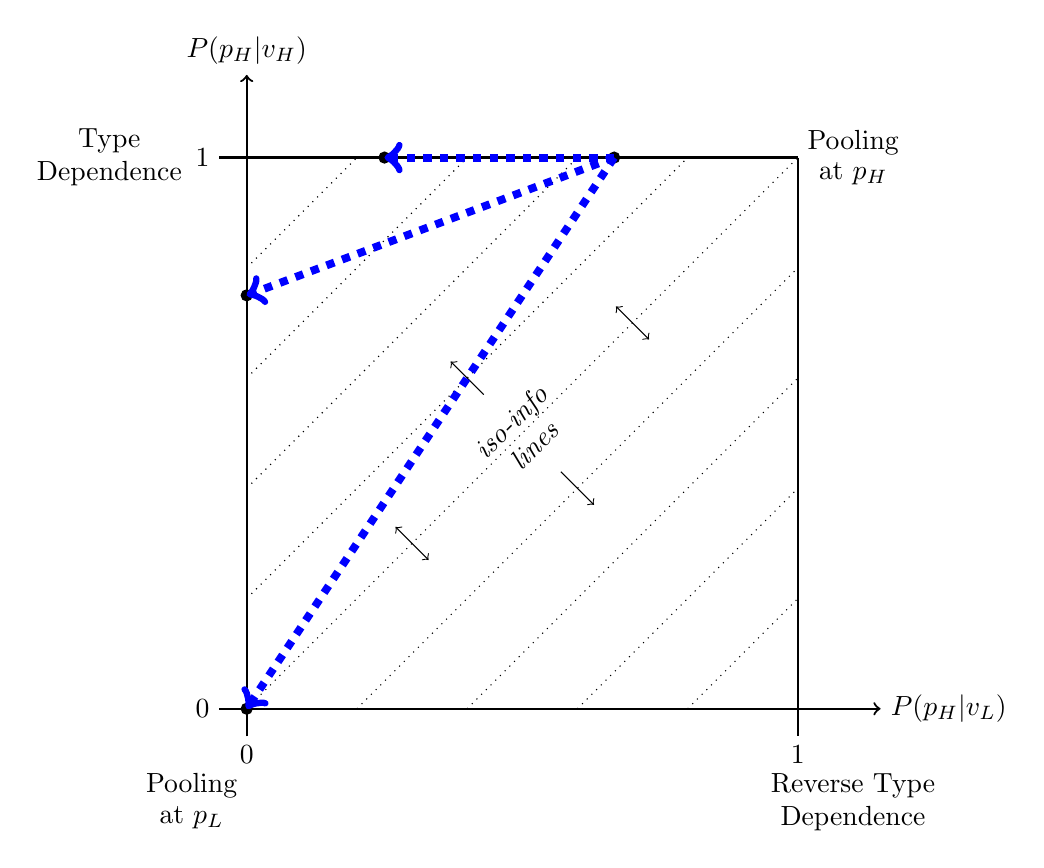
\begin{tikzpicture}[scale=7]

\draw[thick,->] (-0.05,0) -- (1.15,0) node[anchor=west] {$\mathbb{P}(p_H|v_L)$};
\draw[thick,->] (0,-0.05) -- (0,1.15) node[anchor=south] {$\mathbb{P}(p_H|v_H)$};

\draw[thick] (-0.05,1)--(1,1);
\draw[thick] (1,1)--(1,-0.05);

\node[left] at (-0.05,0) {0};
\node[left] at (-0.05,1) {1};
\node[below] at (0,-0.05) {0};
\node[below] at (1,-0.05) {1};

\node[left] at (-0.1,1) {\shortstack{Type \\ Dependence}};
\node[right] at (1,1) {\shortstack{Pooling \\ at $p_H$}};
\node[below] at (1.1,-0.1) {\shortstack{Reverse Type \\ Dependence}};
\node[below] at (-0.1,-0.1) {\shortstack{Pooling \\ at $p_L$}};

\draw[dotted] (0,0)--(1,1);
\draw[dotted] (0,0.2)--(0.8,1);
\draw[dotted] (0,0.4)--(0.6,1);
\draw[dotted] (0,0.6)--(0.4,1);
\draw[dotted] (0,0.8)--(0.2,1);
\draw[dotted] (0.2,0)--(1,0.8);
\draw[dotted] (0.4,0)--(1,0.6);
\draw[dotted] (0.6,0)--(1,0.4);
\draw[dotted] (0.8,0)--(1,0.2);
\draw[<->] (0.73,0.67)--(0.67,0.73);
\draw[<->] (0.33,0.27)--(0.27,0.33);
\draw[->] (0.43,0.57)--(0.37,0.63);
\draw[->] (0.57,0.43)--(0.63,0.37);
\coordinate (P) at (0.5,0.5);
\node[rotate=45] (N) at (P) {\emph{\shortstack{iso-info \\ lines}}};

\node[draw, circle, fill=black, inner sep=0pt, minimum size=4pt] at (0.6666666666666667, 1.0) {};
\node[draw, circle, fill=black, inner sep=0pt, minimum size=4pt] at (0.25, 1.0) {};
\node[draw, circle, fill=black, inner sep=0pt, minimum size=4pt] at (0.0, 0.75) {};
\node[draw, circle, fill=black, inner sep=0pt, minimum size=4pt] at (0.0, 0.0) {};

\draw[line width=0.1cm, dashed, blue,->] (0.6666666666666667, 1.0)--(0.25, 1.0);
\draw[line width=0.1cm, dashed, blue,->] (0.6666666666666667, 1.0)--(0.0, 0.75);
\draw[line width=0.1cm, dashed, blue,->] (0.6666666666666667, 1.0)--(0.0, 0.0);

\end{tikzpicture}
\caption{Potential Seller Strategies as $n$ Increases}
\label{seller_strat_space_2}
\end{figure}
